% Changer les captions pour cacher les références dans la table des figures
\let\caption\oldcaption
\chapter{\'Etat de l'art}

\setcounter{chapter}{1} % Forcer la numérotation pour les compilations à un seul chapitre

\section{Introduction}

L'estimation de la distance à partir des images d'une scène est un problème
fondamental dans la vision artificielle et qui a été étudié depuis longtemps.
Beaucoup d'approches ont été proposées.

Ces approches se répartissent en deux catégories : les méthodes qui sont basées
sur la vision binoculaire et les méthodes basées sur la vision monoculaire.
Les méthodes binoculaires utilisent deux cameras et calculent la distance
en connaissant la position et l'orientation de chaque camera dans la scène
par l'utilisation de principes géométriques comme la triangulation. Les
méthodes basées sur la vision monoculaire qui estiment la distance d'une seule
image par l'extraction de certains caractéristiques de l'image comme la
distribution de la brume et les points de fuite, ou par l'utilisation des
techniques d'apprentissage automatique.

Pour des raisons historiques, la plupart des recherches portant sur l'estimation
de distances ont été basées sur la vision binoculaire ou sur l'utilisation de
plusieurs images, ou encore sur l'utilisation des caractéristiques bien définies
dans la vision monoculaire. Cependant, les dernières années ont connu
l'émergence d'approches basées sur l'apprentissage automatique.
Dans ce chapitre nous présentons ce que nous avons trouvé comme travaux basés
sur l'utilisation des techniques d'apprentissage automatique.

\section{\'Evitement d'obstacles par la vision monoculaire}

L'un des premiers travaux utilisant l'apprentissage automatique et qui ont eu
des résultats satisfaisants est celui de Michels et al.\cite{michels2005high}
qui ont développé une méthode pour permettre à une voiture télécommandée de
naviguer de façon autonome dans un environnement non structuré à une haute
vitesse ($5m/s$).

Dans leur approche ils ont utilisé deux types d'apprentissage : l'apprentissage
supervisé pour estimer les distances des obstacles figurant dans l'image de la
camera, et l'apprentissage par renforcement afin de calculer le degré de
changement de la direction du mouvement. Ce dernier utilise les distances résultantes
du premier apprentissage pour choisir la direction.

Dans la première étape, ils ont construit une plateforme constituée d'un
scanner laser de distances, d'une webcam et d'un ordinateur portable qui commande
ces périphiriques et traite les données qui les génèrent. Cette plateforme se
déplace continuellement dans une forêt pour prendre les photos de
l'environnement et les mesures de distance respectives.

\begin{figure}[H]
\begin{center}
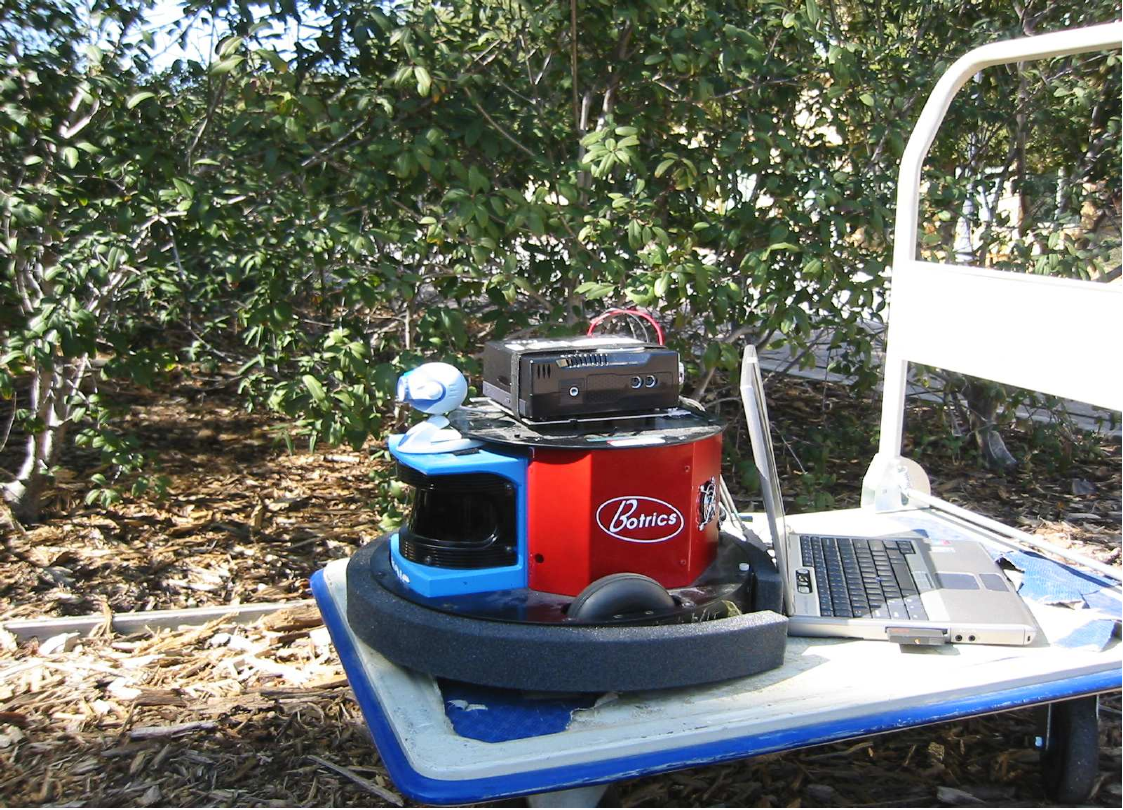
\includegraphics[width=0.7\textwidth]{HighSpeedObstacleAvoidanceRig}
\caption{La plateforme qui prend les mesures et les photos}
\end{center}
\end{figure}

Chaque image collectée est divisée en 16 bandes verticales dont chacune correspond
à une distance. Chaque bande est transformée en un vecteur de caractéristiques
généré à partir de la texture. Ensuite, une \keyword{régression linéaire} est
appliquée pour générer les paramètres du modèle qui prédit les distances en
utilisant les vecteurs de caractéristiques avec les distances correspondantes.
Les données utilisées sont des images réelles combinées avec des images synthétisées.
Par la suite, un simulateur est utilisé afin d'entraîner par renforcement un
autre modèle qui permet de décider l'angle de déviation.

Enfin, les deux modèles ont été implémentés pour contrôler le véhicule à
distance. Ce véhicule dispose d'un émetteur qui lui permet d'envoyer l'image
capturée vers l'ordinateur qui calcule les distances, choisit le degré de
déviation et l'utilise pour commander le véhicule. La figure suivante présente
une séquence d'images montrant le changement de direction du véhicule lors de
la détection d'un obstacle (un arbuste). Le premier rang montre les positions
du véhicule, le second est sa vision, et le dernier représente les distances
estimées des obstacles.

\begin{figure}[H]
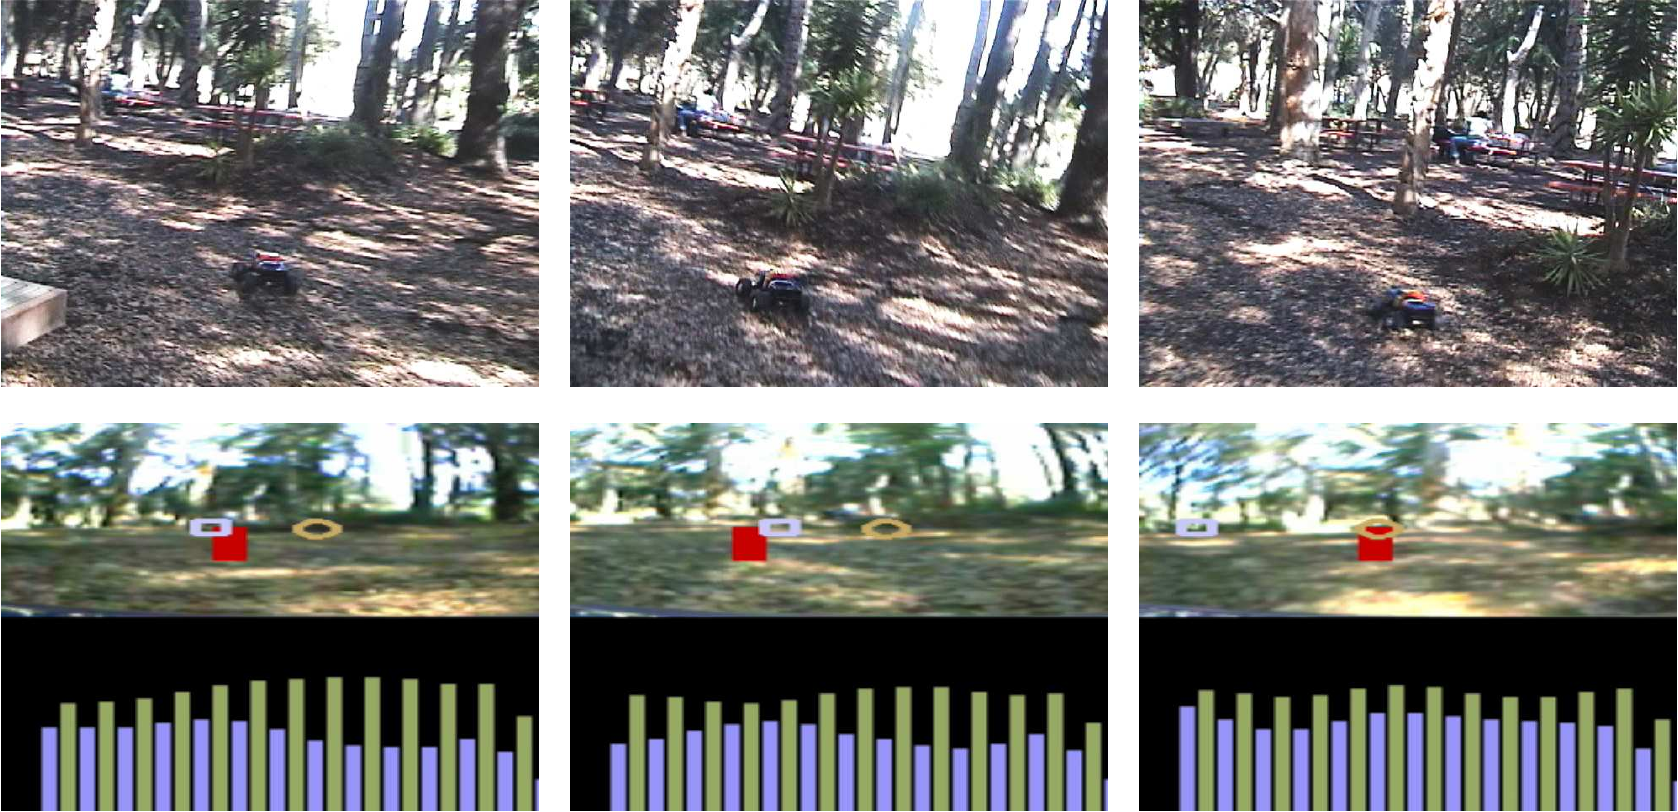
\includegraphics[width=\textwidth]{RC_car}
\caption{Une séquence d'images montrant l'évitement d'un obstacle}
\end{figure}

\section{Apprentissage de la profondeur d'une seule image}

Saxena et al.\cite{saxena2005learning} ont travaillé sur l'estimation de la
profondeur d'une seule image par l'utilisation d'un apprentissage supervisé.
Les images et les cartes de profondeur sont collectées à partir des scènes de
l'extérieur fortement destructurées contenant plusieurs objets (arbres, bâtiments, etc).

Contrairement à Michels and all, les images sont divisées en de petites
pièces servant à calculer les vecteurs de caractéristiques sur différentes
échelles en utilisant des masques de convolution.

\begin{figure}[H]
\begin{center}
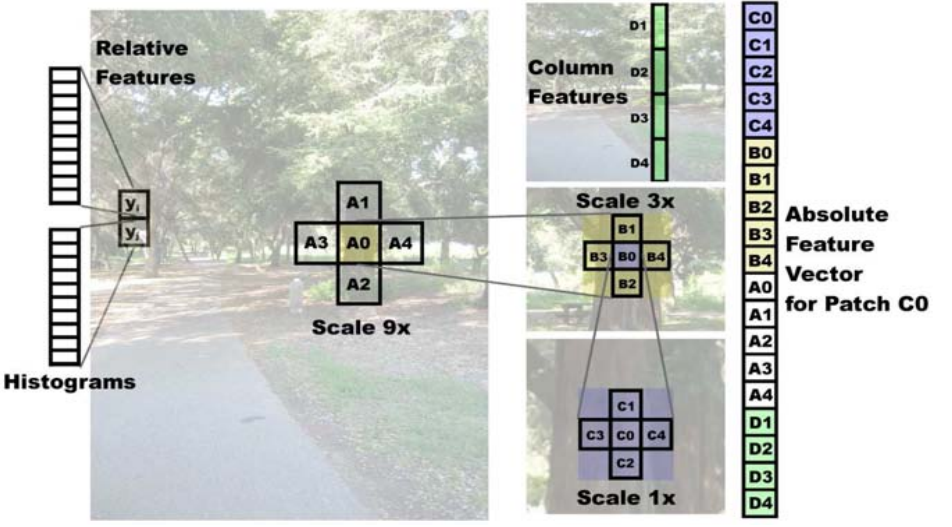
\includegraphics[width=0.75\textwidth]{FeaturesVectorScales}
\caption{Le vecteur de caractéristiques à  différentes échelles}
\end{center}
\end{figure}

De plus, il ont choisi la technique du \keyword{champ aléatoire de Markov} comme
méthode d'apprentissage car elle est un modèle probabiliste permettant de
prendre en considération les corrélations existantes entre pièces adjacentes.
Ils ont commencé par la variante gaussienne du modèle, puis ils ont
basculé vers la laplacienne vu qu'elle est la plus adaptée à ce problème.
La figure suivante présente quelques résultats de leurs expériences, la première
colonne représente l'image, la deuxième c'est la carte des profondeurs réelles, et
les deux dernières sont les cartes de profondeurs générées par le modèle gaussien
et le modèle laplacien respectivement.

\begin{figure}[H]
\begin{center}
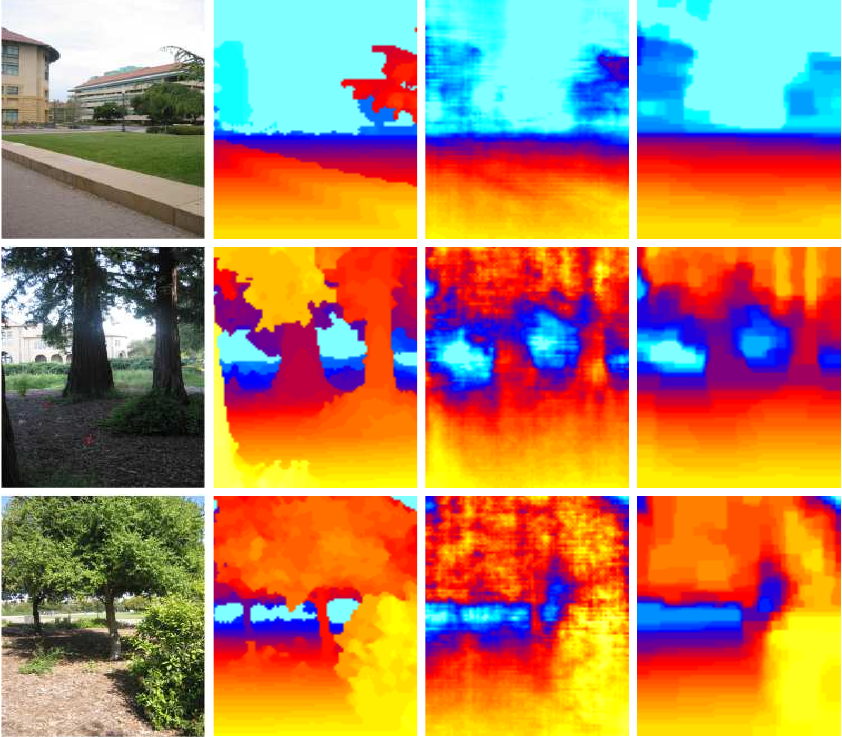
\includegraphics[width=0.75\textwidth]{DepthLearningResults}
\caption{Quelques résultats de l'apprentissage de profondeur}
\end{center}
\end{figure}

Dans un autre travail, Saxena et al.\cite{saxena2009make3d} ont aussi utilisé les
\keyword{champs aléatoires de Markov}
pour estimer la structure 3D détaillée d'une scène. De même, leur travail -qui
s'appelle \keyword{Make3D}- repose sur l'utilisation d'apprentissage supervisé et
sur la vision monoculaire. Ils ont décomposé chaque image en un ensemble de
triangles appelés \keyword{superpixels} où chacun représente une surface planaire.
Les informations de la profondeur sont utilisées de la même manière que dans les
travaux précédents, mais en ajoutant des contraintes géométriques permettant de
traiter plus de cas. Ils ont réussi à transformer plusieurs images 2D en
images 3D. Ils ont aussi étendu leur projet pour utiliser d'autres informations
quand c'est possible, comme les relations entre les objets dans une seule image, ou
la différence de vues pour une photo. La figure suivante montre des photos
utilisées dans leurs tests avec les résultats obtenus.

\begin{figure}[H]
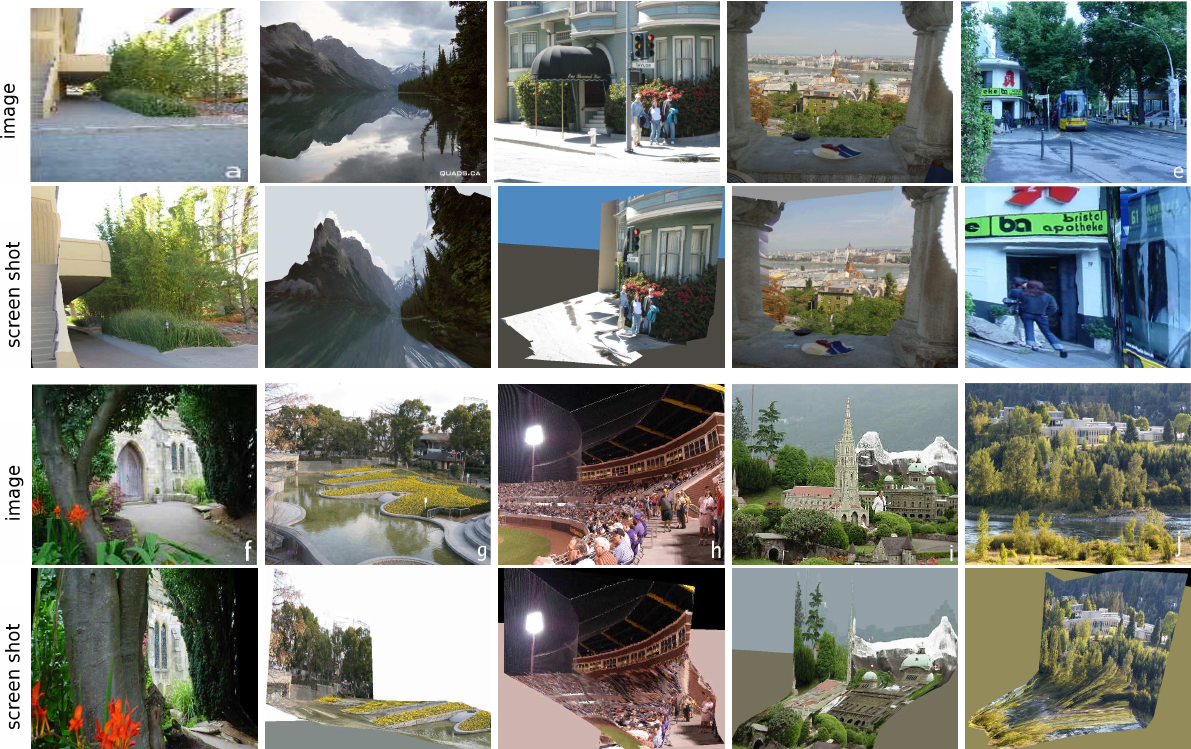
\includegraphics[width=\textwidth]{make3D_tests}
\caption{Quelques images transformées en 3D avec Make3D}
\end{figure}

\section{Les réseaux de neurones convolutionels pour l'estimation de la profondeur}

Un des travaux récents qui ont utilisé les \keyword{réseaux de neurones convolutionels}
pour l'estimation de profondeur est celui de Eigen et al.\cite{eigen2014depth}.

L'approche consiste à développer un réseau de neurones convolutionel consitué de
deux niveaux. Le premier prédit la profondeur à un niveau global, tandis que le
deuxième applique des raffinements successifs afin de générer une carte des
profondeurs plus précise. Les deux niveaux acceptent l'image originale comme
entrée. De plus, la sortie du premier niveau est fournie comme entrée pour
le deuxième.

Ils ont entraîné ce modèle par les ensembles de données de \keyword{NYU v2} qui
contient des scènes d'intérieur de maison, et de \keyword{KITTI} qui est un ensemble
de scènes d'extérieur. Les résultats obtenus après l'apprentissage étaient
généralement meilleurs que ceux de \keyword{Make3D}, et cela est dû à la
structure multi-échelles du réseau qui permet de combiner la vue globale avec les
vues locales sur l'image.

\begin{figure}[H]
\begin{center}
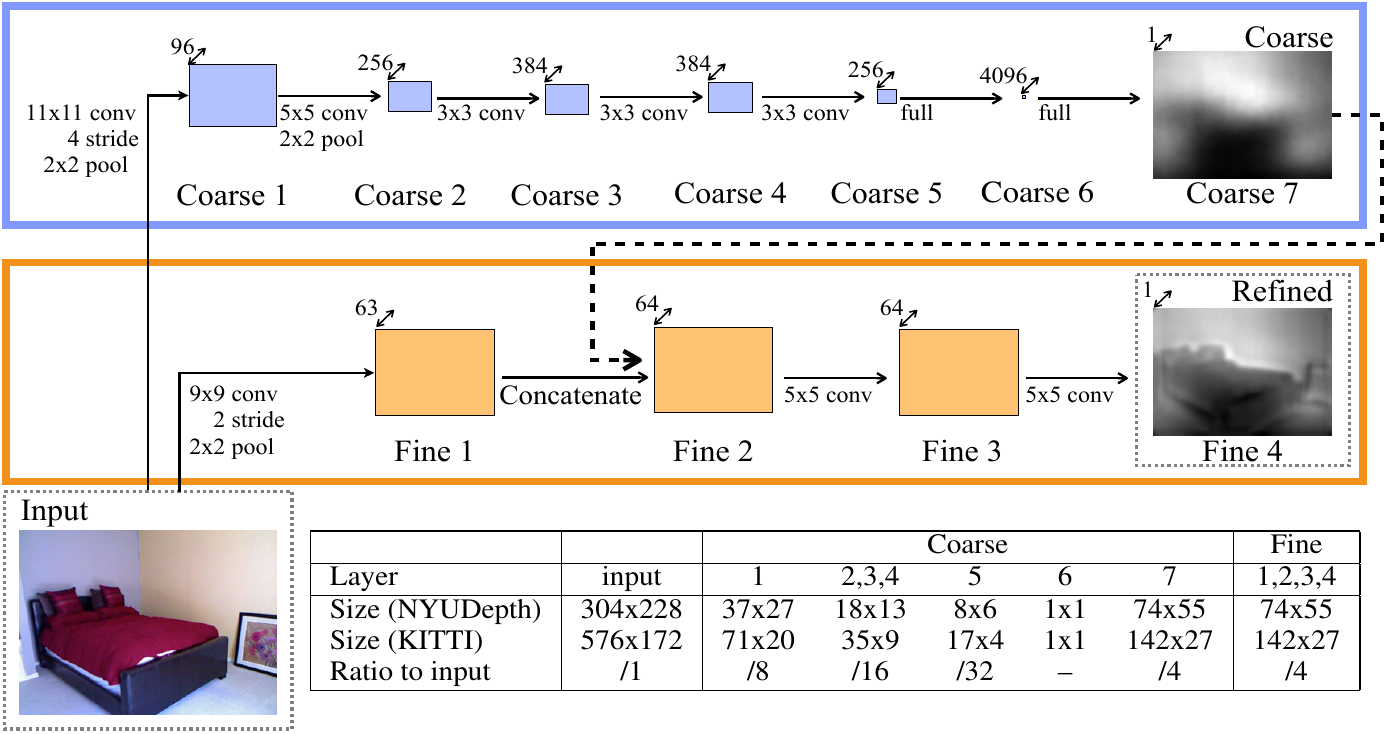
\includegraphics[width=0.6\textwidth]{Double_CNN_Architecture}
\caption{L'architecture du réseau à deux niveaux}
\end{center}
\end{figure}

\vspace{-1em}

Dans un travail ultérieur, Eigen et Fergus\cite{eigen2015predicting} ont étendu
le modèle précédent par l'ajout de deux autres fonctionnalitées : l'estimation
de la normale de chaque surface et l'étiquetage sémantique. Ils ont gardé le
principe de réseaux multi-échelles qui ne nécessite aucun prétraitement de bas
niveau.

La nouvelle architecture de ce modèle est formée de trois sous réseaux
convolutionels dont le résultat de chacun et l'image originale sont alimentés
au suivant, les sous-réseaux étant plus profonds que ceux du travail précédent.
Le premier permet de prédire des caractéristiques globales sur toute l'image.
Le second produit des prédictions d'un niveau moyen de détails en intégrant les
informations du premier. Le dernier affine ces prédictions pour générer une
sortie à un haut niveau de détails en utilisant toutes les informations précédentes.

\vspace{1em}

\begin{figure}[H]
\begin{center}
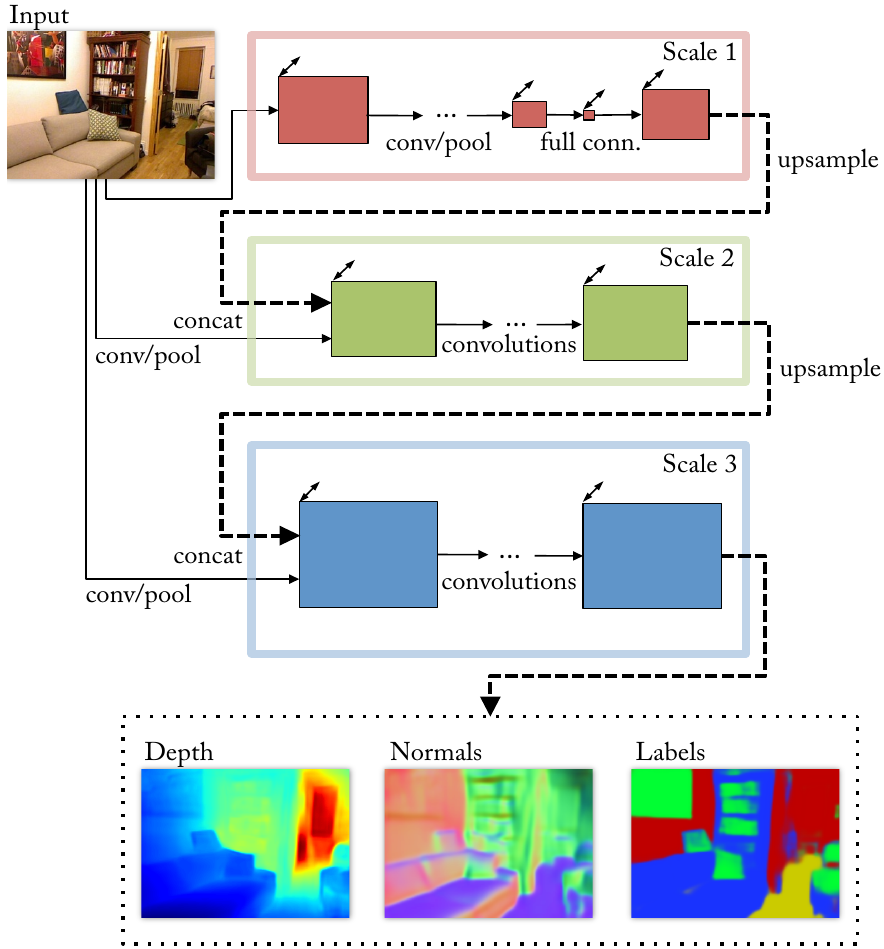
\includegraphics[width=0.5\textwidth]{CNN_Multi_Architecture}
\caption{L'architecture du réseau à trois niveaux}
\end{center}
\end{figure}

\section{Les champs de neurones convolutionels}

Liu et al.\cite{liu2015deep} ont créé un modèle hybride qui bénifice de la combinaison
des \keyword{réseaux de neurones convolutionels} avec les \keyword{champs aléatoires
conditionnels} (CRF) pour l'estimation de la profondeur. Le modèle est composé de deux
parties : une partie qui calcule les similarités par paires entre les
\keyword{superpixels} voisins qui sont transmis à une couche entièrement connectée,
et l'autre partie qui est un réseau convolutionel constitué de cinq couches
convolutionelles suivies par quatre autres entièrement connectées. Le résultat
de chacune de ces deux parties est fourni à la couche finale qui calcule la
probabilité de chaque profondeur en utilisant la formule de CRF.

\begin{figure}[H]
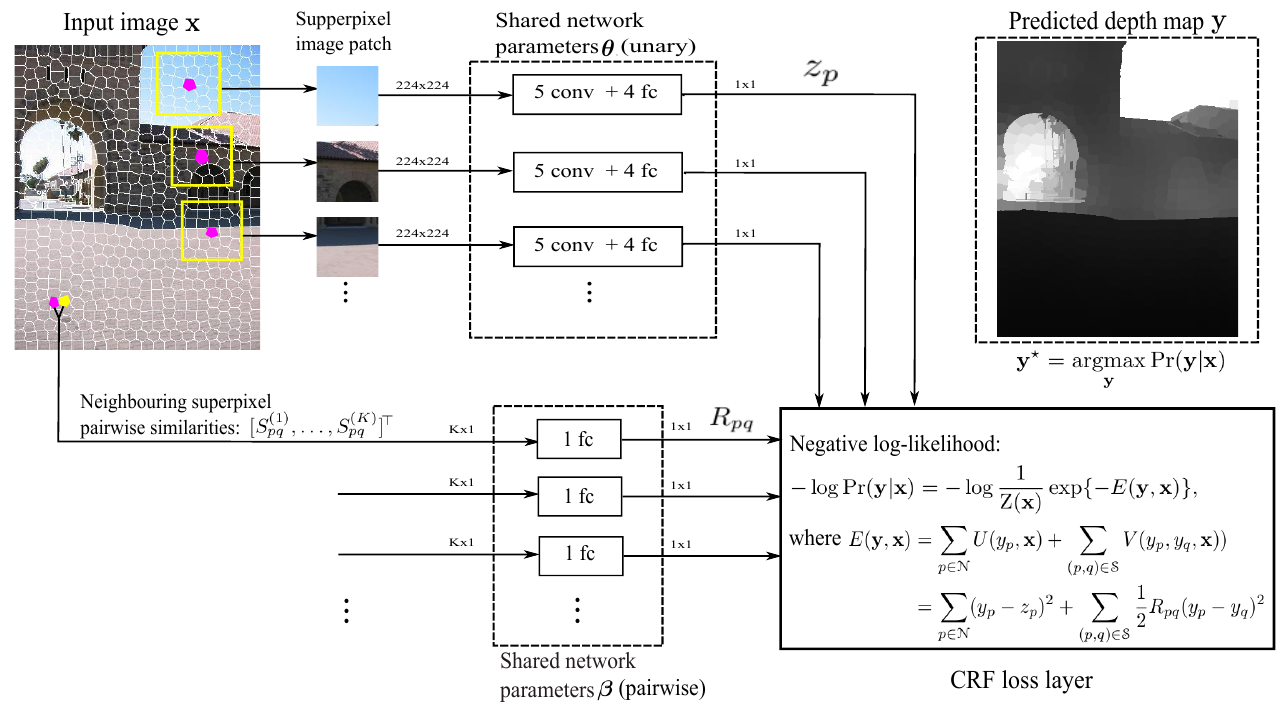
\includegraphics[width=\textwidth]{CRF_CNN_Architecture}
\caption{L'architecture globale du champ de neurones convolutionel}
\end{figure}

L'apprentissage a été effectué après avoir initialisé les couches par les poids
d'\keyword{ImageNet} en utilisant l'ensemble de données de \keyword{Make3D} et de
\keyword{NYU v2}. Ce travail a dépassé toutes les méthodes existantes pour
ces deux ensembles de données.

\section{Conclusion}

Dans ce chapitre nous avons présenté quelques travaux antérieurs concernant
l'estimation de distances ou de profondeurs à partir d'une seule image.
Toutes ces méthodes utilisent les ensembles de données contenant des cartes de
profondeurs générées à partir des scanners laser (comme SICK et Microsoft Kinect)
car ils sont très précis pour calculer la distance d'un point.
Cependant, ils ont quelques inconvénients, comme leur poids qui ne peut pas être négligeable
et leur sensibilité à la lumière du soleil qui peut fausser les calculs, ce que
les rend peu pratiques pour l'utilisation dans les appareils qui peuvent être
exposés aux rayons solaires. De plus, il sont relativement coûteux.

A notre connaissance, tous les projets d'estimation de distances précédents
n'ont utilisé que les scanners lasers. De ce fait, nous avons essayé d'utiliser
une autre option : les capteurs ultrasoniques. Bien que leur précision soit
relativement plus faible que celle des scanners laser et que leur taux d'erreur
puisse être élevé dans les scènes contenant des objets avec des surfaces
irrégulières, ils ont des avantages comme leur légèreté et leur insensibilité
à la lumière, et de plus, leur coût est très faible.

Dans le chapitre suivant nous présenterons les parties matérielles et logicielles
formant notre projet qui est un robot constiué de plusieurs composants et
programmé pour pouvoir se déplacer en prenant des photos de l'environnement
avec les distances respectives.
